\section{Bias plots for the base finetuned model} \label{sec:bias_plots_base}

The faithfulness and plausibility metrics of the base fine-tuned model obtained using ferret are depicted in \autoref{fig:ferret-base}. The explainers are listed on the x-axis. \enquote{Ig} is shorthand for the integrated gradient explainer. \enquote{Igmby} is the integrated gradient explainer multiplied by the inputs.

\begin{figure*}[t!]
    \centering
    \begin{subfigure}{0.49\textwidth}
        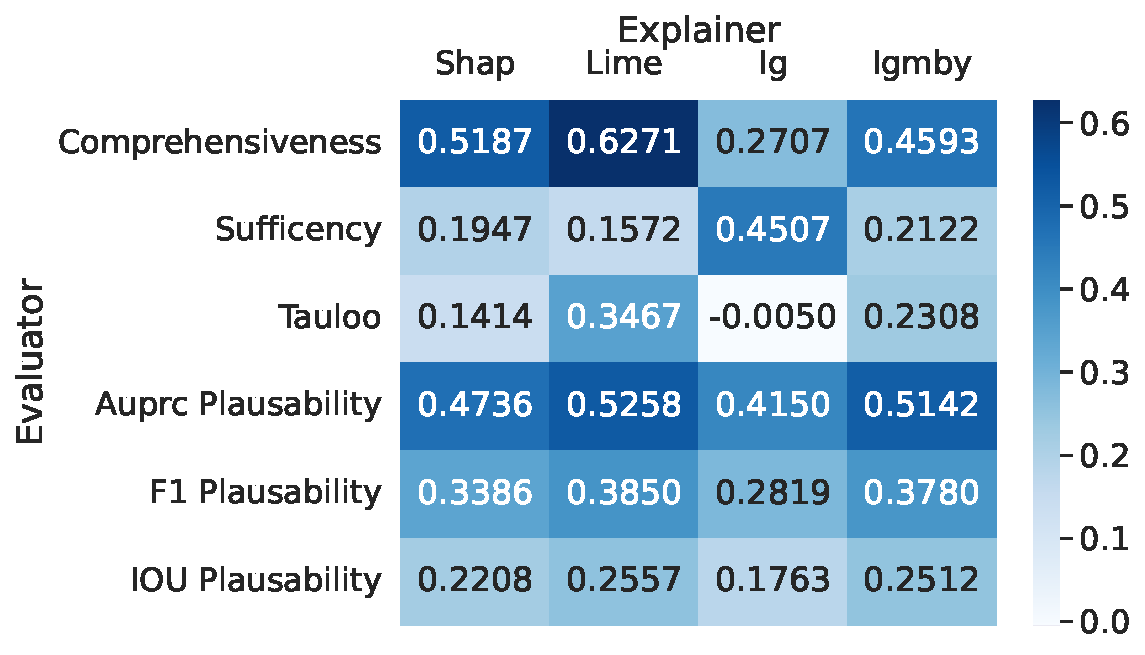
\includegraphics[width=\textwidth]{./images/ferret_heatmaps_phenomena/default_mnli/synonym.pdf}
        \caption{Synonyms}
    \end{subfigure}
    \begin{subfigure}{0.49\textwidth}
        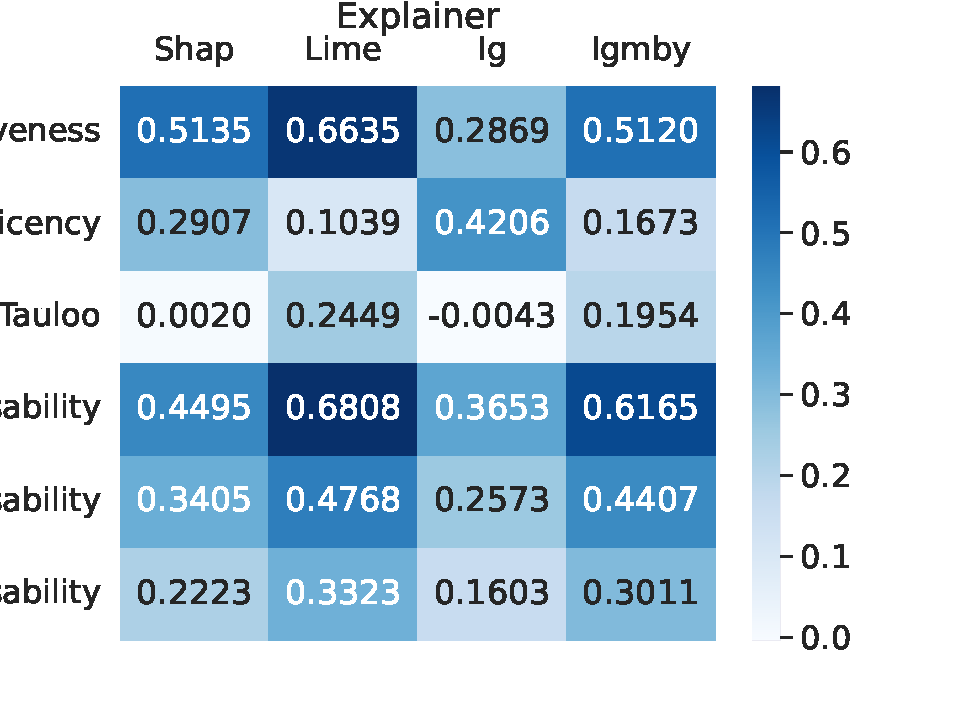
\includegraphics[width=\textwidth]{./images/ferret_heatmaps_phenomena/default_mnli/antonym.pdf}
        \caption{Antonyms}
    \end{subfigure}
    \begin{subfigure}{0.49\textwidth}
        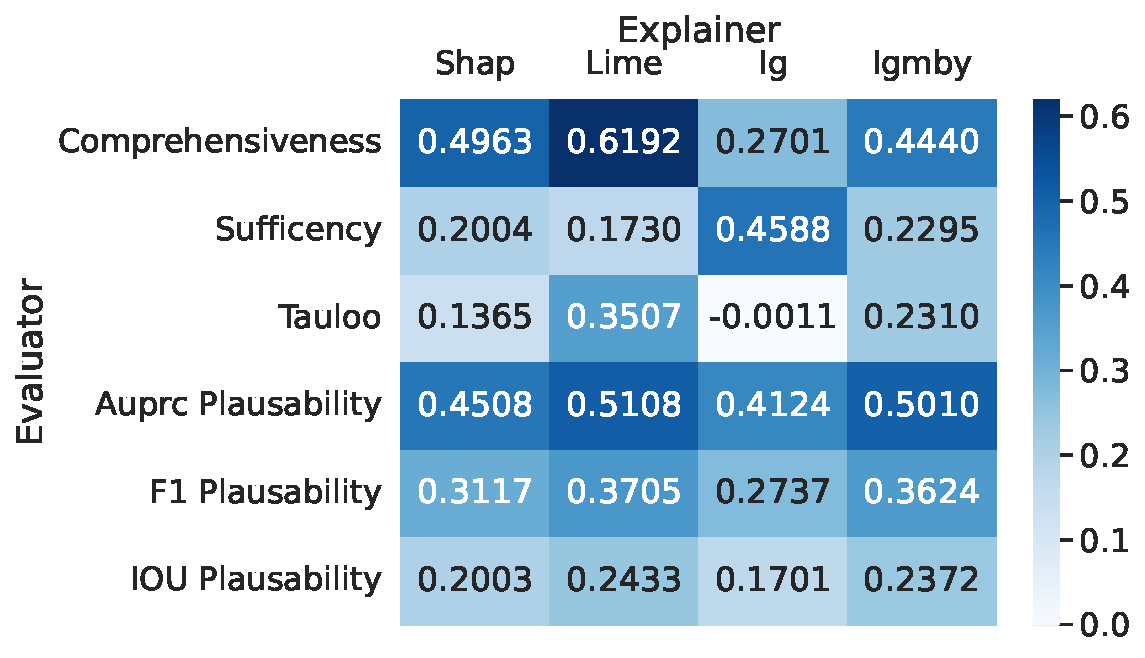
\includegraphics[width=\textwidth]{./images/ferret_heatmaps_phenomena/default_mnli/hypernym.pdf}
        \caption{Hypernyms}
    \end{subfigure}
    \begin{subfigure}{0.49\textwidth}
        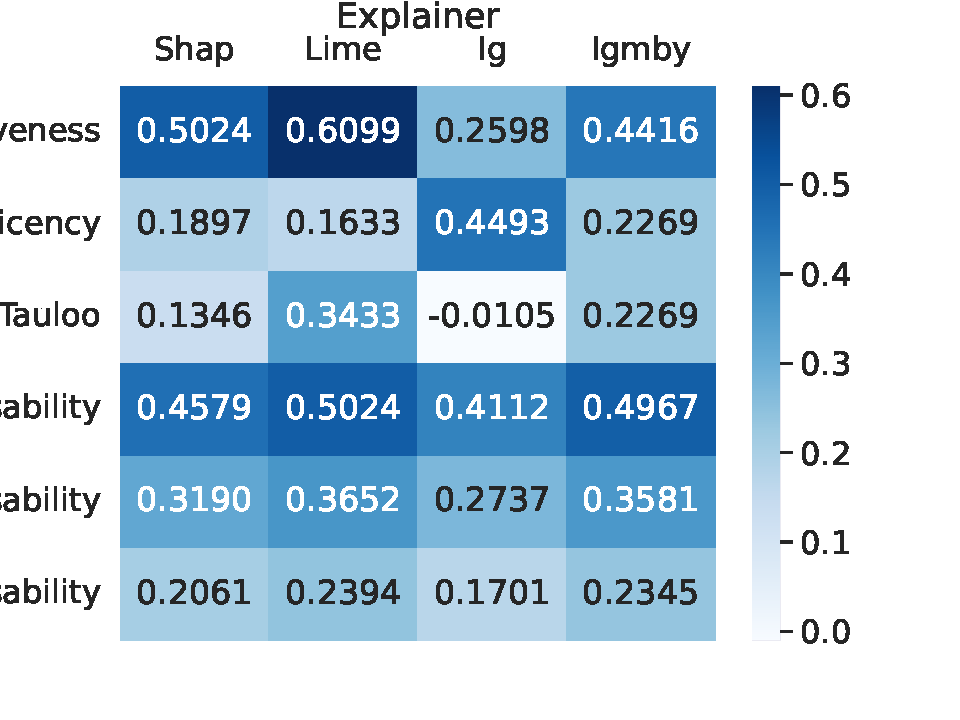
\includegraphics[width=\textwidth]{./images/ferret_heatmaps_phenomena/default_mnli/hyponym.pdf}
        \caption{Hyponyms}
    \end{subfigure}
    \begin{subfigure}{0.49\textwidth}
        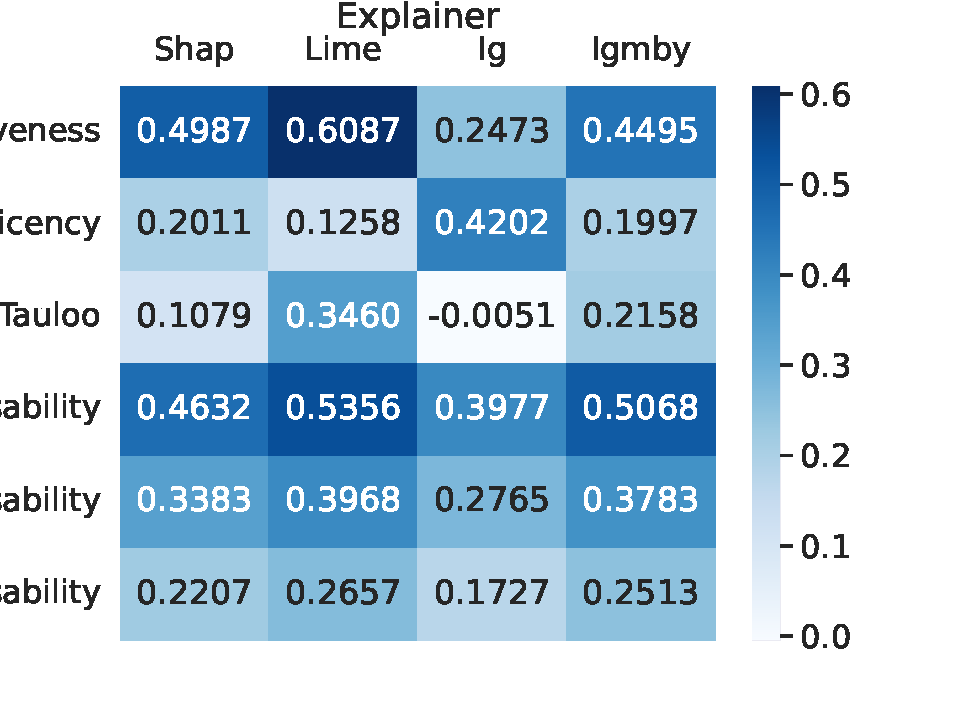
\includegraphics[width=\textwidth]{./images/ferret_heatmaps_phenomena/default_mnli/co_hyponym.pdf}
        \caption{Co-Hyponyms}
    \end{subfigure}
    \begin{subfigure}{0.49\textwidth}
        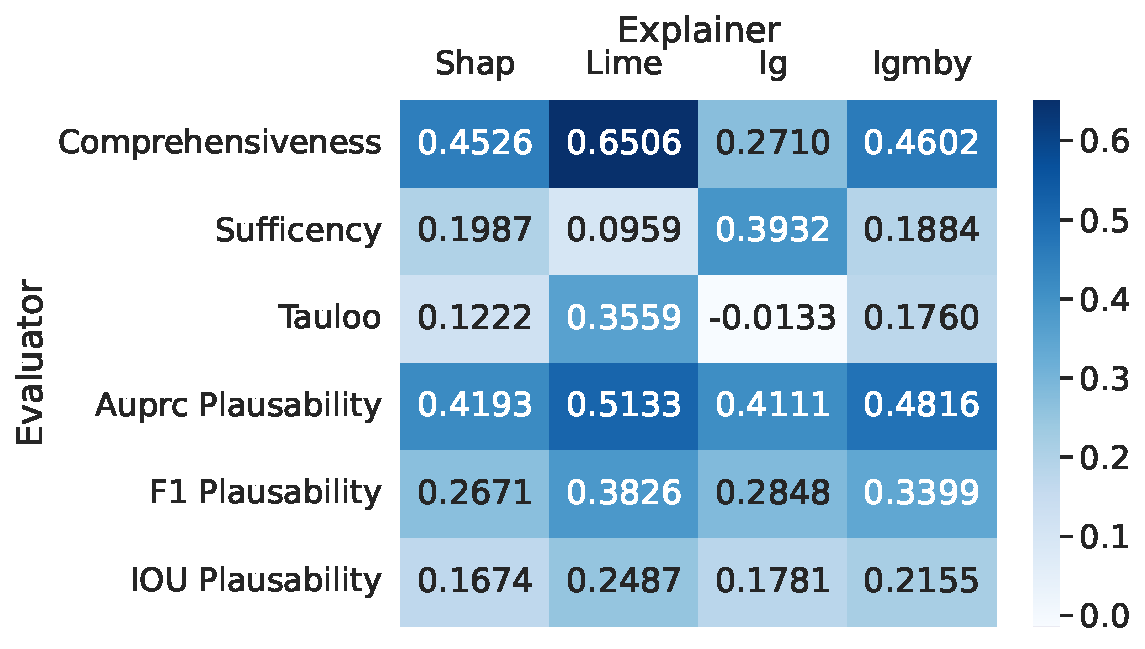
\includegraphics[width=\textwidth]{./images/ferret_heatmaps_phenomena/default_mnli/quantifiers.pdf}
        \caption{Quantifiers}
    \end{subfigure}
    \begin{subfigure}{0.49\textwidth}
        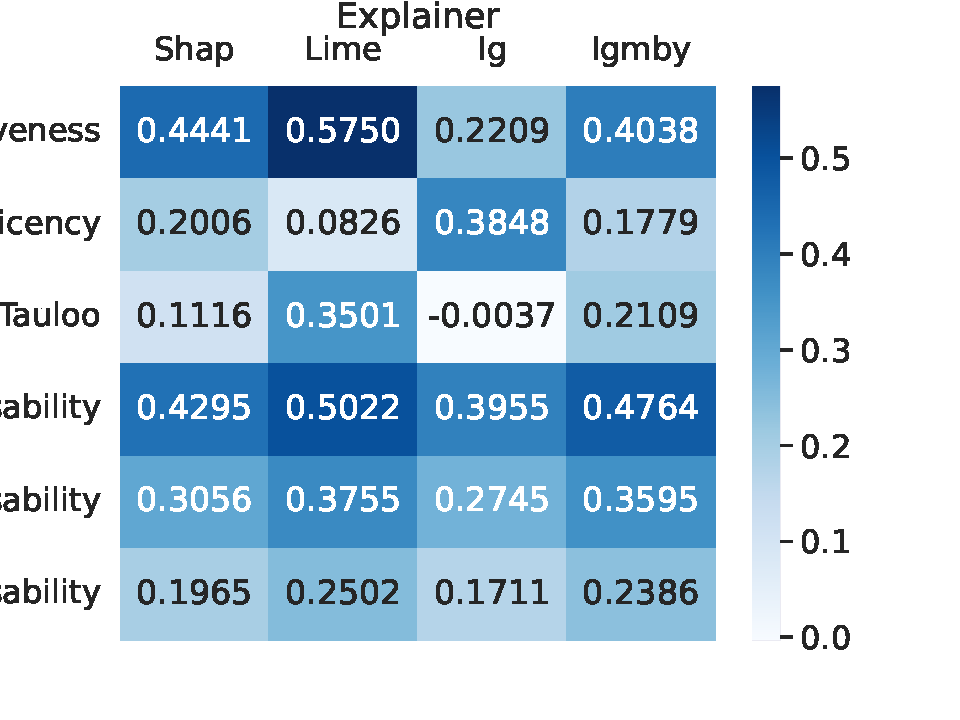
\includegraphics[width=\textwidth]{./images/ferret_heatmaps_phenomena/default_mnli/numericals.pdf}
        \caption{Numerals}
    \end{subfigure}
    \caption{Faithfulness and plausibility of the base model measured on \acs{e-SNLI} filtered for linguistic phenomena}
    \label{fig:ferret-base}
\end{figure*}

\section{Bias plots for the filtered finetuned model} \label{sec:bias_plots_filtered}

The faithfulness and plausibility metrics of the model \enquote{Filtered 3/3 longer} obtained using ferret are depicted in \autoref{fig:ferret-base}. The explainers are listed on the x-axis. \enquote{Ig} is shorthand for the integrated gradient explainer. \enquote{Igmby} is the integrated gradient explainer multiplied by the inputs.

\begin{figure*}[t!]
    \centering
    \begin{subfigure}{0.49\textwidth}
        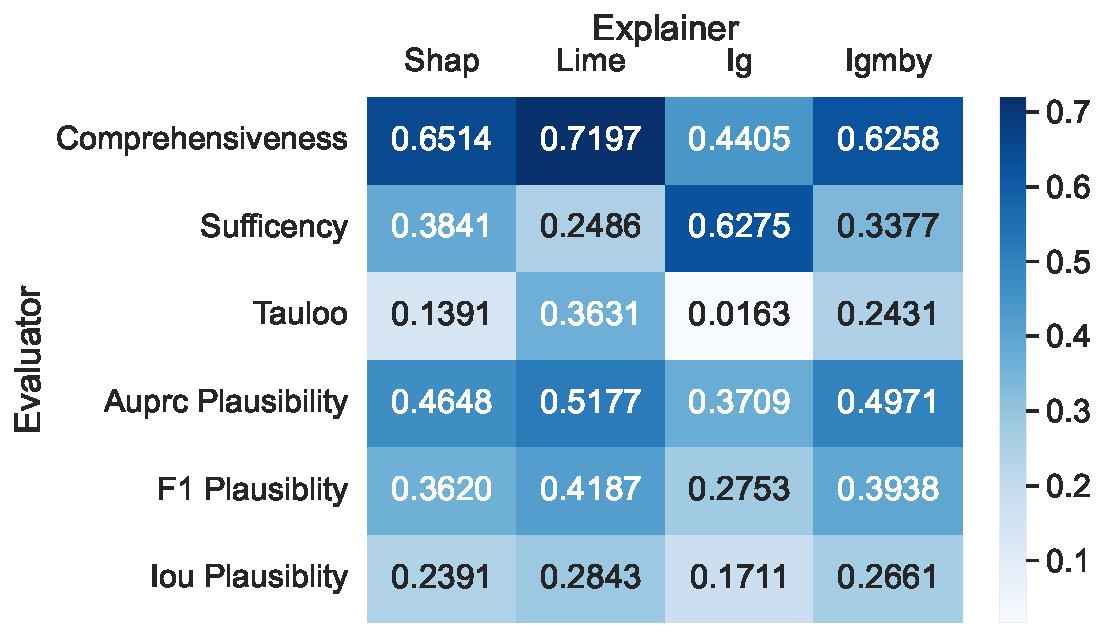
\includegraphics[width=\textwidth]{./images/ferret_heatmaps_phenomena/filtered_3_3_longer/synonym.pdf}
        \caption{Synonyms}
    \end{subfigure}
    \begin{subfigure}{0.49\textwidth}
        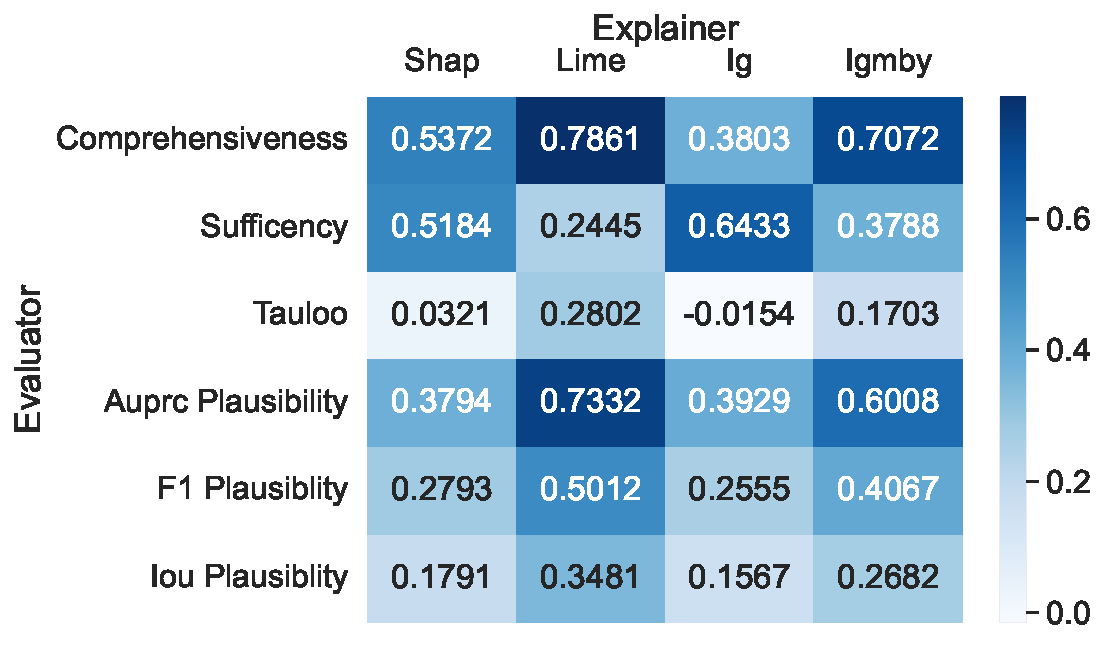
\includegraphics[width=\textwidth]{./images/ferret_heatmaps_phenomena/filtered_3_3_longer/antonym.pdf}
        \caption{Antonyms}
    \end{subfigure}
    \begin{subfigure}{0.49\textwidth}
        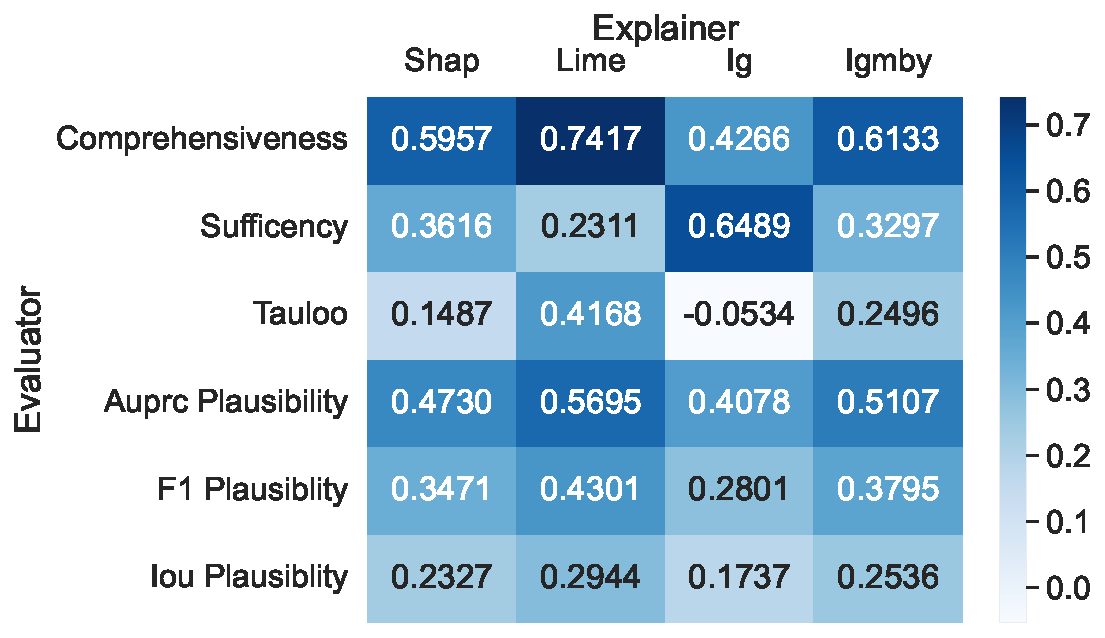
\includegraphics[width=\textwidth]{./images/ferret_heatmaps_phenomena/filtered_3_3_longer/hypernym.pdf}
        \caption{Hypernyms}
    \end{subfigure}
    \begin{subfigure}{0.49\textwidth}
        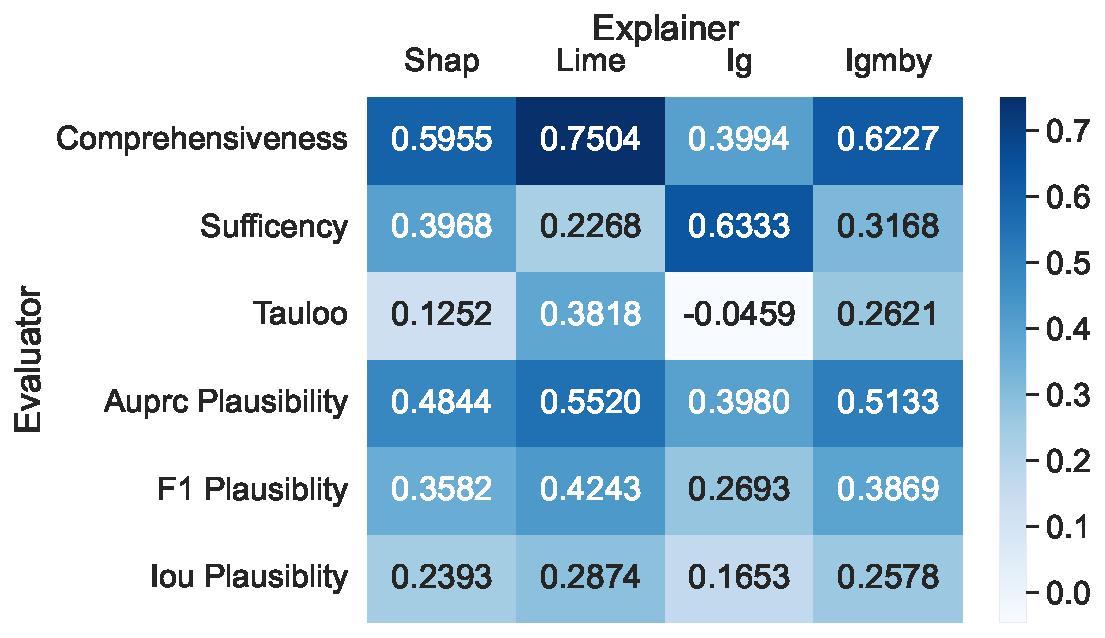
\includegraphics[width=\textwidth]{./images/ferret_heatmaps_phenomena/filtered_3_3_longer/hyponym.pdf}
        \caption{Hyponyms}
    \end{subfigure}
    \begin{subfigure}{0.49\textwidth}
        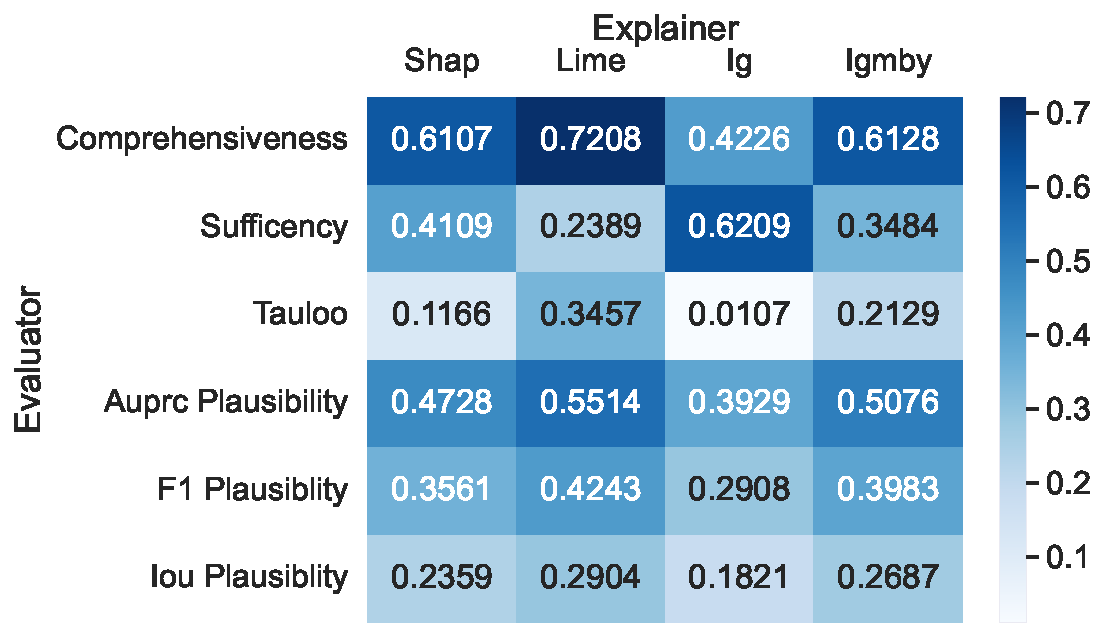
\includegraphics[width=\textwidth]{./images/ferret_heatmaps_phenomena/filtered_3_3_longer/co_hyponym.pdf}
        \caption{Co-Hyponyms}
    \end{subfigure}
    \begin{subfigure}{0.49\textwidth}
        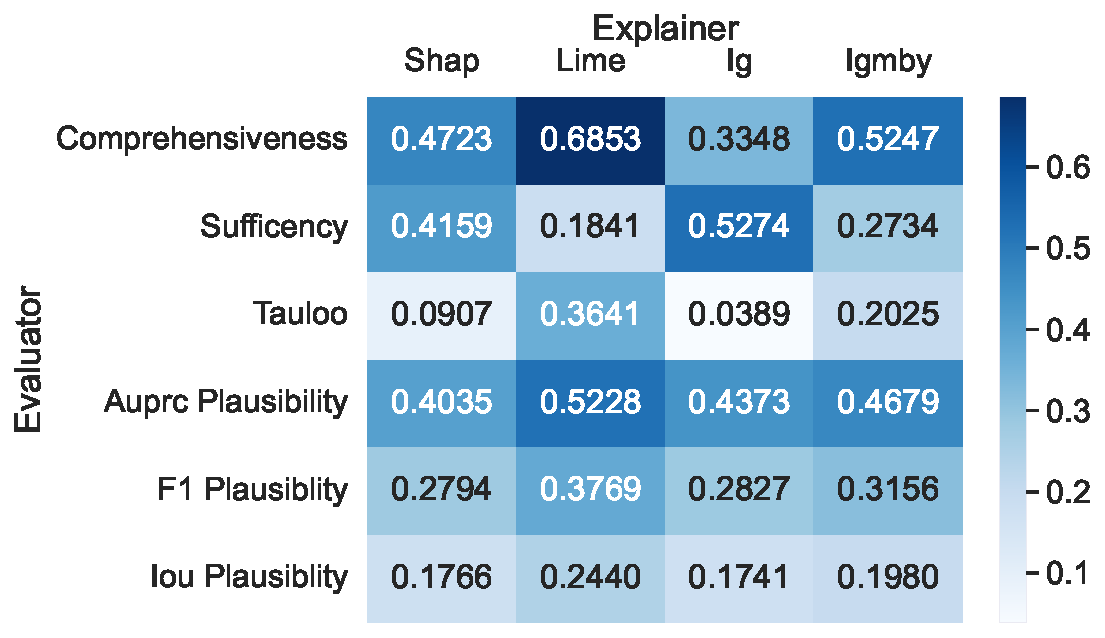
\includegraphics[width=\textwidth]{./images/ferret_heatmaps_phenomena/filtered_3_3_longer/quantifiers.pdf}
        \caption{Quantifiers}
    \end{subfigure}
    \begin{subfigure}{0.49\textwidth}
        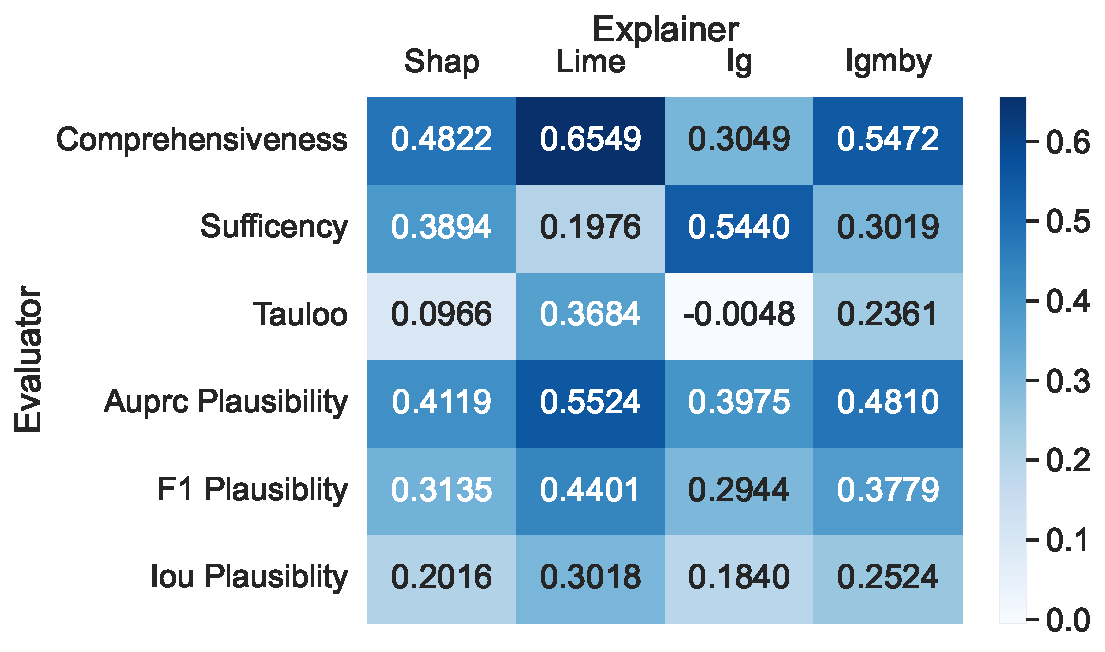
\includegraphics[width=\textwidth]{./images/ferret_heatmaps_phenomena/filtered_3_3_longer/numericals.pdf}
        \caption{Numerals}
    \end{subfigure}
    \caption{Faithfulness and plausibility of the \enquote{Filtered 3/3 longer} model measured on \acs{e-SNLI} filtered for linguistic phenomena}
    \label{fig:ferret-filtered}
\end{figure*}